\documentclass[1p]{elsarticle_modified}
%\bibliographystyle{elsarticle-num}

%\usepackage[colorlinks]{hyperref}
%\usepackage{abbrmath_seonhwa} %\Abb, \Ascr, \Acal ,\Abf, \Afrak
\usepackage{amsfonts}
\usepackage{amssymb}
\usepackage{amsmath}
\usepackage{amsthm}
\usepackage{scalefnt}
\usepackage{amsbsy}
\usepackage{kotex}
\usepackage{caption}
\usepackage{subfig}
\usepackage{color}
\usepackage{graphicx}
\usepackage{xcolor} %% white, black, red, green, blue, cyan, magenta, yellow
\usepackage{float}
\usepackage{setspace}
\usepackage{hyperref}

\usepackage{tikz}
\usetikzlibrary{arrows}

\usepackage{multirow}
\usepackage{array} % fixed length table
\usepackage{hhline}

%%%%%%%%%%%%%%%%%%%%%
\makeatletter
\renewcommand*\env@matrix[1][\arraystretch]{%
	\edef\arraystretch{#1}%
	\hskip -\arraycolsep
	\let\@ifnextchar\new@ifnextchar
	\array{*\c@MaxMatrixCols c}}
\makeatother %https://tex.stackexchange.com/questions/14071/how-can-i-increase-the-line-spacing-in-a-matrix
%%%%%%%%%%%%%%%

\usepackage[normalem]{ulem}

\newcommand{\msout}[1]{\ifmmode\text{\sout{\ensuremath{#1}}}\else\sout{#1}\fi}
%SOURCE: \msout is \stkout macro in https://tex.stackexchange.com/questions/20609/strikeout-in-math-mode

\newcommand{\cancel}[1]{
	\ifmmode
	{\color{red}\msout{#1}}
	\else
	{\color{red}\sout{#1}}
	\fi
}

\newcommand{\add}[1]{
	{\color{blue}\uwave{#1}}
}

\newcommand{\replace}[2]{
	\ifmmode
	{\color{red}\msout{#1}}{\color{blue}\uwave{#2}}
	\else
	{\color{red}\sout{#1}}{\color{blue}\uwave{#2}}
	\fi
}

\newcommand{\Sol}{\mathcal{S}} %segment
\newcommand{\D}{D} %diagram
\newcommand{\A}{\mathcal{A}} %arc


%%%%%%%%%%%%%%%%%%%%%%%%%%%%%5 test

\def\sl{\operatorname{\textup{SL}}(2,\Cbb)}
\def\psl{\operatorname{\textup{PSL}}(2,\Cbb)}
\def\quan{\mkern 1mu \triangleright \mkern 1mu}

\theoremstyle{definition}
\newtheorem{thm}{Theorem}[section]
\newtheorem{prop}[thm]{Proposition}
\newtheorem{lem}[thm]{Lemma}
\newtheorem{ques}[thm]{Question}
\newtheorem{cor}[thm]{Corollary}
\newtheorem{defn}[thm]{Definition}
\newtheorem{exam}[thm]{Example}
\newtheorem{rmk}[thm]{Remark}
\newtheorem{alg}[thm]{Algorithm}

\newcommand{\I}{\sqrt{-1}}
\begin{document}

%\begin{frontmatter}
%
%\title{Boundary parabolic representations of knots up to 8 crossings}
%
%%% Group authors per affiliation:
%\author{Yunhi Cho} 
%\address{Department of Mathematics, University of Seoul, Seoul, Korea}
%\ead{yhcho@uos.ac.kr}
%
%
%\author{Seonhwa Kim} %\fnref{s_kim}}
%\address{Center for Geometry and Physics, Institute for Basic Science, Pohang, 37673, Korea}
%\ead{ryeona17@ibs.re.kr}
%
%\author{Hyuk Kim}
%\address{Department of Mathematical Sciences, Seoul National University, Seoul 08826, Korea}
%\ead{hyukkim@snu.ac.kr}
%
%\author{Seokbeom Yoon}
%\address{Department of Mathematical Sciences, Seoul National University, Seoul, 08826,  Korea}
%\ead{sbyoon15@snu.ac.kr}
%
%\begin{abstract}
%We find all boundary parabolic representation of knots up to 8 crossings.
%
%\end{abstract}
%\begin{keyword}
%    \MSC[2010] 57M25 
%\end{keyword}
%
%\end{frontmatter}

%\linenumbers
%\tableofcontents
%
\newcommand\colored[1]{\textcolor{white}{\rule[-0.35ex]{0.8em}{1.4ex}}\kern-0.8em\color{red} #1}%
%\newcommand\colored[1]{\textcolor{white}{ #1}\kern-2.17ex	\textcolor{white}{ #1}\kern-1.81ex	\textcolor{white}{ #1}\kern-2.15ex\color{red}#1	}

{\Large $\underline{12n_{0010}~(K12n_{0010})}$}

\setlength{\tabcolsep}{10pt}
\renewcommand{\arraystretch}{1.6}
\vspace{1cm}\begin{tabular}{m{100pt}>{\centering\arraybackslash}m{274pt}}
\multirow{5}{120pt}{
	\centering
	\includegraphics[width=112pt]{../../../GIT/diagram.site/Diagrams/png/2099_12n_0010.png}\\
\ \ \ A knot diagram\footnotemark}&
\allowdisplaybreaks
\textbf{Linearized knot diagam} \\
\cline{2-2}
 &
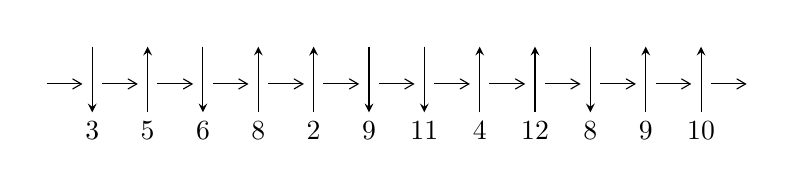
\begin{tikzpicture}[x=20pt, y=17pt]
	% nodes
	\node (C0) at (0, 0) {};
	\node (C1) at (1, 0) {};
	\node (C1U) at (1, +1) {};
	\node (C1D) at (1, -1) {3};

	\node (C2) at (2, 0) {};
	\node (C2U) at (2, +1) {};
	\node (C2D) at (2, -1) {5};

	\node (C3) at (3, 0) {};
	\node (C3U) at (3, +1) {};
	\node (C3D) at (3, -1) {6};

	\node (C4) at (4, 0) {};
	\node (C4U) at (4, +1) {};
	\node (C4D) at (4, -1) {8};

	\node (C5) at (5, 0) {};
	\node (C5U) at (5, +1) {};
	\node (C5D) at (5, -1) {2};

	\node (C6) at (6, 0) {};
	\node (C6U) at (6, +1) {};
	\node (C6D) at (6, -1) {9};

	\node (C7) at (7, 0) {};
	\node (C7U) at (7, +1) {};
	\node (C7D) at (7, -1) {11};

	\node (C8) at (8, 0) {};
	\node (C8U) at (8, +1) {};
	\node (C8D) at (8, -1) {4};

	\node (C9) at (9, 0) {};
	\node (C9U) at (9, +1) {};
	\node (C9D) at (9, -1) {12};

	\node (C10) at (10, 0) {};
	\node (C10U) at (10, +1) {};
	\node (C10D) at (10, -1) {8};

	\node (C11) at (11, 0) {};
	\node (C11U) at (11, +1) {};
	\node (C11D) at (11, -1) {9};

	\node (C12) at (12, 0) {};
	\node (C12U) at (12, +1) {};
	\node (C12D) at (12, -1) {10};
	\node (C13) at (13, 0) {};

	% arrows
	\draw[->,>={angle 60}]
	(C0) edge (C1) (C1) edge (C2) (C2) edge (C3) (C3) edge (C4) (C4) edge (C5) (C5) edge (C6) (C6) edge (C7) (C7) edge (C8) (C8) edge (C9) (C9) edge (C10) (C10) edge (C11) (C11) edge (C12) (C12) edge (C13) ;	\draw[->,>=stealth]
	(C1U) edge (C1D) (C2D) edge (C2U) (C3U) edge (C3D) (C4D) edge (C4U) (C5D) edge (C5U) (C6U) edge (C6D) (C7U) edge (C7D) (C8D) edge (C8U) (C9D) edge (C9U) (C10U) edge (C10D) (C11D) edge (C11U) (C12D) edge (C12U) ;
	\end{tikzpicture} \\
\hhline{~~} \\& 
\textbf{Solving Sequence} \\ \cline{2-2} 
 &
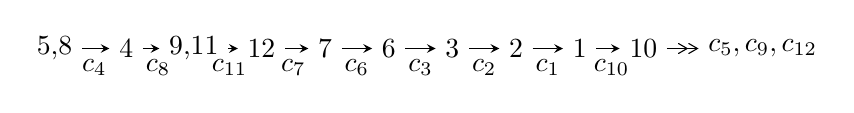
\begin{tikzpicture}[x=23pt, y=7pt]
	% node
	\node (A0) at (-1/8, 0) {5,8};
	\node (A1) at (1, 0) {4};
	\node (A2) at (33/16, 0) {9,11};
	\node (A3) at (25/8, 0) {12};
	\node (A4) at (33/8, 0) {7};
	\node (A5) at (41/8, 0) {6};
	\node (A6) at (49/8, 0) {3};
	\node (A7) at (57/8, 0) {2};
	\node (A8) at (65/8, 0) {1};
	\node (A9) at (73/8, 0) {10};
	\node (C1) at (1/2, -1) {$c_{4}$};
	\node (C2) at (3/2, -1) {$c_{8}$};
	\node (C3) at (21/8, -1) {$c_{11}$};
	\node (C4) at (29/8, -1) {$c_{7}$};
	\node (C5) at (37/8, -1) {$c_{6}$};
	\node (C6) at (45/8, -1) {$c_{3}$};
	\node (C7) at (53/8, -1) {$c_{2}$};
	\node (C8) at (61/8, -1) {$c_{1}$};
	\node (C9) at (69/8, -1) {$c_{10}$};
	\node (A10) at (11, 0) {$c_{5},c_{9},c_{12}$};

	% edge
	\draw[->,>=stealth]	
	(A0) edge (A1) (A1) edge (A2) (A2) edge (A3) (A3) edge (A4) (A4) edge (A5) (A5) edge (A6) (A6) edge (A7) (A7) edge (A8) (A8) edge (A9) ;
	\draw[->>,>={angle 60}]	
	(A9) edge (A10);
\end{tikzpicture} \\ 

\end{tabular} \\

\footnotetext{
The image of knot diagram is generated by the software ``\textbf{Draw programme}" developed by Andrew Bartholomew(\url{http://www.layer8.co.uk/maths/draw/index.htm\#Running-draw}), where we modified some parts for our purpose(\url{https://github.com/CATsTAILs/LinksPainter}).
}\phantom \\ \newline 
\centering \textbf{Ideals for irreducible components\footnotemark of $X_{\text{par}}$} 
 
\begin{align*}
I^u_{1}&=\langle 
373570485293358 u^{28}+1033333880231479 u^{27}+\cdots+1737205994835979 b-46103598198659,\\
\phantom{I^u_{1}}&\phantom{= \langle  }-452869533551973 u^{28}-703336104853671 u^{27}+\cdots+1737205994835979 a-136865573763131,\\
\phantom{I^u_{1}}&\phantom{= \langle  }u^{29}+2 u^{28}+\cdots- u-1\rangle \\
I^u_{2}&=\langle 
- u^3+b- u-1,\;a,\;u^4+u^2+u+1\rangle \\
I^u_{3}&=\langle 
- u^5+u^4-2 u^3+2 u^2+b-2 u+2,\;a,\;u^6- u^5+2 u^4-2 u^3+2 u^2-2 u+1\rangle \\
\\
\end{align*}
\raggedright * 3 irreducible components of $\dim_{\mathbb{C}}=0$, with total 39 representations.\\
\footnotetext{All coefficients of polynomials are rational numbers. But the coefficients are sometimes approximated in decimal forms when there is not enough margin.}
\newpage
\renewcommand{\arraystretch}{1}
\centering \section*{I. $I^u_{1}= \langle 3.74\times10^{14} u^{28}+1.03\times10^{15} u^{27}+\cdots+1.74\times10^{15} b-4.61\times10^{13},\;-4.53\times10^{14} u^{28}-7.03\times10^{14} u^{27}+\cdots+1.74\times10^{15} a-1.37\times10^{14},\;u^{29}+2 u^{28}+\cdots- u-1 \rangle$}
\flushleft \textbf{(i) Arc colorings}\\
\begin{tabular}{m{7pt} m{180pt} m{7pt} m{180pt} }
\flushright $a_{5}=$&$\begin{pmatrix}1\\0\end{pmatrix}$ \\
\flushright $a_{8}=$&$\begin{pmatrix}0\\u\end{pmatrix}$ \\
\flushright $a_{4}=$&$\begin{pmatrix}1\\u^2\end{pmatrix}$ \\
\flushright $a_{9}=$&$\begin{pmatrix}u\\u^3+u\end{pmatrix}$ \\
\flushright $a_{11}=$&$\begin{pmatrix}0.260688 u^{28}+0.404866 u^{27}+\cdots+1.65378 u+0.0787849\\-0.215041 u^{28}-0.594825 u^{27}+\cdots+2.17523 u+0.0265389\end{pmatrix}$ \\
\flushright $a_{12}=$&$\begin{pmatrix}u\\-0.574992 u^{28}-1.22877 u^{27}+\cdots+1.37727 u+0.0642647\end{pmatrix}$ \\
\flushright $a_{7}=$&$\begin{pmatrix}0.281422 u^{28}+0.665341 u^{27}+\cdots+0.425718 u-0.328077\\-0.300941 u^{28}-0.245733 u^{27}+\cdots+0.372268 u-0.413702\end{pmatrix}$ \\
\flushright $a_{6}=$&$\begin{pmatrix}0.0992626 u^{28}+0.229078 u^{27}+\cdots+0.144178 u-0.116511\\-0.422114 u^{28}-0.580655 u^{27}+\cdots-0.163376 u-0.274080\end{pmatrix}$ \\
\flushright $a_{3}=$&$\begin{pmatrix}0.0599722 u^{28}+0.00259463 u^{27}+\cdots-0.0401153 u+1.59959\\0.138580 u^{28}+0.0401668 u^{27}+\cdots-0.139073 u+1.22534\end{pmatrix}$ \\
\flushright $a_{2}=$&$\begin{pmatrix}-0.0786083 u^{28}-0.0375722 u^{27}+\cdots+0.0989573 u+0.374257\\0.138580 u^{28}+0.0401668 u^{27}+\cdots-0.139073 u+1.22534\end{pmatrix}$ \\
\flushright $a_{1}=$&$\begin{pmatrix}0.493107 u^{28}+0.774647 u^{27}+\cdots+0.437369 u+0.188122\\0.393844 u^{28}+0.545569 u^{27}+\cdots+0.293191 u+0.304633\end{pmatrix}$ \\
\flushright $a_{10}=$&$\begin{pmatrix}0.260688 u^{28}+0.404866 u^{27}+\cdots+1.65378 u+0.0787849\\-0.314304 u^{28}-0.823903 u^{27}+\cdots+2.03105 u+0.143050\end{pmatrix}$\\&\end{tabular}
\flushleft \textbf{(ii) Obstruction class $= -1$}\\~\\
\flushleft \textbf{(iii) Cusp Shapes $= -\frac{7883435024310839}{1737205994835979} u^{28}-\frac{14219216887312602}{1737205994835979} u^{27}+\cdots+\frac{21942781332157203}{1737205994835979} u+\frac{8811379112410107}{1737205994835979}$}\\~\\
\newpage\renewcommand{\arraystretch}{1}
\flushleft \textbf{(iv) u-Polynomials at the component}\newline \\
\begin{tabular}{m{50pt}|m{274pt}}
Crossings & \hspace{64pt}u-Polynomials at each crossing \\
\hline $$\begin{aligned}c_{1}\end{aligned}$$&$\begin{aligned}
&u^{29}+12 u^{28}+\cdots+u-1
\end{aligned}$\\
\hline $$\begin{aligned}c_{2},c_{5}\end{aligned}$$&$\begin{aligned}
&u^{29}+2 u^{28}+\cdots+u-1
\end{aligned}$\\
\hline $$\begin{aligned}c_{3}\end{aligned}$$&$\begin{aligned}
&u^{29}-2 u^{28}+\cdots+120 u-36
\end{aligned}$\\
\hline $$\begin{aligned}c_{4},c_{8}\end{aligned}$$&$\begin{aligned}
&u^{29}-2 u^{28}+\cdots- u+1
\end{aligned}$\\
\hline $$\begin{aligned}c_{6}\end{aligned}$$&$\begin{aligned}
&u^{29}-10 u^{28}+\cdots-469083 u+52489
\end{aligned}$\\
\hline $$\begin{aligned}c_{7},c_{10}\end{aligned}$$&$\begin{aligned}
&u^{29}-5 u^{28}+\cdots-3072 u-1024
\end{aligned}$\\
\hline $$\begin{aligned}c_{9},c_{11},c_{12}\end{aligned}$$&$\begin{aligned}
&u^{29}+11 u^{28}+\cdots-30 u^2-1
\end{aligned}$\\
\hline
\end{tabular}\\~\\
\newpage\renewcommand{\arraystretch}{1}
\flushleft \textbf{(v) Riley Polynomials at the component}\newline \\
\begin{tabular}{m{50pt}|m{274pt}}
Crossings & \hspace{64pt}Riley Polynomials at each crossing \\
\hline $$\begin{aligned}c_{1}\end{aligned}$$&$\begin{aligned}
&y^{29}+12 y^{28}+\cdots+85 y-1
\end{aligned}$\\
\hline $$\begin{aligned}c_{2},c_{5}\end{aligned}$$&$\begin{aligned}
&y^{29}+12 y^{28}+\cdots+y-1
\end{aligned}$\\
\hline $$\begin{aligned}c_{3}\end{aligned}$$&$\begin{aligned}
&y^{29}+12 y^{28}+\cdots-12456 y-1296
\end{aligned}$\\
\hline $$\begin{aligned}c_{4},c_{8}\end{aligned}$$&$\begin{aligned}
&y^{29}+30 y^{27}+\cdots+y-1
\end{aligned}$\\
\hline $$\begin{aligned}c_{6}\end{aligned}$$&$\begin{aligned}
&y^{29}+92 y^{28}+\cdots-44517246691 y-2755095121
\end{aligned}$\\
\hline $$\begin{aligned}c_{7},c_{10}\end{aligned}$$&$\begin{aligned}
&y^{29}+63 y^{28}+\cdots+3670016 y-1048576
\end{aligned}$\\
\hline $$\begin{aligned}c_{9},c_{11},c_{12}\end{aligned}$$&$\begin{aligned}
&y^{29}-51 y^{28}+\cdots-60 y-1
\end{aligned}$\\
\hline
\end{tabular}\\~\\
\newpage\flushleft \textbf{(vi) Complex Volumes and Cusp Shapes}
$$\begin{array}{c|c|c}  
\text{Solutions to }I^u_{1}& \I (\text{vol} + \sqrt{-1}CS) & \text{Cusp shape}\\
 \hline 
\begin{aligned}
u &= \phantom{-}0.269747 + 0.997117 I \\
a &= -0.080093 + 0.634791 I \\
b &= -0.459723 - 0.451799 I\end{aligned}
 & -3.76543 - 0.40137 I & -7.74784 + 0.84155 I \\ \hline\begin{aligned}
u &= \phantom{-}0.269747 - 0.997117 I \\
a &= -0.080093 - 0.634791 I \\
b &= -0.459723 + 0.451799 I\end{aligned}
 & -3.76543 + 0.40137 I & -7.74784 - 0.84155 I \\ \hline\begin{aligned}
u &= -0.520591 + 0.795499 I \\
a &= \phantom{-}0.040524 + 0.941049 I \\
b &= \phantom{-}1.201380 + 0.062565 I\end{aligned}
 & \phantom{-}0.03144 - 1.92773 I & \phantom{-}1.38434 + 3.11728 I \\ \hline\begin{aligned}
u &= -0.520591 - 0.795499 I \\
a &= \phantom{-}0.040524 - 0.941049 I \\
b &= \phantom{-}1.201380 - 0.062565 I\end{aligned}
 & \phantom{-}0.03144 + 1.92773 I & \phantom{-}1.38434 - 3.11728 I \\ \hline\begin{aligned}
u &= -0.896581 + 0.315451 I \\
a &= -1.90204 + 1.76626 I \\
b &= -0.36922 + 3.53096 I\end{aligned}
 & \phantom{-}4.34061 - 5.06790 I & \phantom{-}7.76076 + 6.40955 I \\ \hline\begin{aligned}
u &= -0.896581 - 0.315451 I \\
a &= -1.90204 - 1.76626 I \\
b &= -0.36922 - 3.53096 I\end{aligned}
 & \phantom{-}4.34061 + 5.06790 I & \phantom{-}7.76076 - 6.40955 I \\ \hline\begin{aligned}
u &= \phantom{-}0.888576 + 0.223844 I \\
a &= \phantom{-}2.22962 + 1.30457 I \\
b &= \phantom{-}1.34311 + 2.77938 I\end{aligned}
 & \phantom{-}4.83420 - 0.14491 I & \phantom{-}9.33140 - 0.02437 I \\ \hline\begin{aligned}
u &= \phantom{-}0.888576 - 0.223844 I \\
a &= \phantom{-}2.22962 - 1.30457 I \\
b &= \phantom{-}1.34311 - 2.77938 I\end{aligned}
 & \phantom{-}4.83420 + 0.14491 I & \phantom{-}9.33140 + 0.02437 I \\ \hline\begin{aligned}
u &= \phantom{-}0.586489 + 0.957504 I \\
a &= -0.302708 + 0.858093 I \\
b &= -1.34326 - 0.63754 I\end{aligned}
 & -1.89724 + 6.62062 I & -1.77451 - 5.81131 I \\ \hline\begin{aligned}
u &= \phantom{-}0.586489 - 0.957504 I \\
a &= -0.302708 - 0.858093 I \\
b &= -1.34326 + 0.63754 I\end{aligned}
 & -1.89724 - 6.62062 I & -1.77451 + 5.81131 I\\
 \hline 
 \end{array}$$\newpage$$\begin{array}{c|c|c}  
\text{Solutions to }I^u_{1}& \I (\text{vol} + \sqrt{-1}CS) & \text{Cusp shape}\\
 \hline 
\begin{aligned}
u &= -0.538341 + 0.454787 I \\
a &= -0.661454 + 0.909012 I \\
b &= \phantom{-}0.67192 + 1.39992 I\end{aligned}
 & \phantom{-}0.49621 - 1.44403 I & \phantom{-}2.32169 + 4.35214 I \\ \hline\begin{aligned}
u &= -0.538341 - 0.454787 I \\
a &= -0.661454 - 0.909012 I \\
b &= \phantom{-}0.67192 - 1.39992 I\end{aligned}
 & \phantom{-}0.49621 + 1.44403 I & \phantom{-}2.32169 - 4.35214 I \\ \hline\begin{aligned}
u &= -0.454661 + 0.440048 I \\
a &= -0.603679 + 0.541804 I \\
b &= -0.128589 + 1.154160 I\end{aligned}
 & \phantom{-}0.61760 - 1.38123 I & \phantom{-}3.89803 + 4.67424 I \\ \hline\begin{aligned}
u &= -0.454661 - 0.440048 I \\
a &= -0.603679 - 0.541804 I \\
b &= -0.128589 - 1.154160 I\end{aligned}
 & \phantom{-}0.61760 + 1.38123 I & \phantom{-}3.89803 - 4.67424 I \\ \hline\begin{aligned}
u &= \phantom{-}0.571853 + 0.250420 I \\
a &= \phantom{-}0.590811 + 0.162782 I \\
b &= \phantom{-}0.832609 + 0.563271 I\end{aligned}
 & -0.23394 - 2.60554 I & \phantom{-}1.51395 + 2.58658 I \\ \hline\begin{aligned}
u &= \phantom{-}0.571853 - 0.250420 I \\
a &= \phantom{-}0.590811 - 0.162782 I \\
b &= \phantom{-}0.832609 - 0.563271 I\end{aligned}
 & -0.23394 + 2.60554 I & \phantom{-}1.51395 - 2.58658 I \\ \hline\begin{aligned}
u &= \phantom{-}0.600458\phantom{ +0.000000I} \\
a &= \phantom{-}1.34216\phantom{ +0.000000I} \\
b &= -0.231076\phantom{ +0.000000I}\end{aligned}
 & \phantom{-}2.41354\phantom{ +0.000000I} & \phantom{-}4.07200\phantom{ +0.000000I} \\ \hline\begin{aligned}
u &= -0.092427 + 0.519848 I \\
a &= -0.242741 + 1.091430 I \\
b &= \phantom{-}0.12625 + 2.93959 I\end{aligned}
 & \phantom{-}2.03975 + 2.27000 I & -9.41057 + 5.26980 I \\ \hline\begin{aligned}
u &= -0.092427 - 0.519848 I \\
a &= -0.242741 - 1.091430 I \\
b &= \phantom{-}0.12625 - 2.93959 I\end{aligned}
 & \phantom{-}2.03975 - 2.27000 I & -9.41057 - 5.26980 I \\ \hline\begin{aligned}
u &= -1.10611 + 1.07911 I \\
a &= \phantom{-}0.66217 - 1.55771 I \\
b &= -4.13956 - 3.94336 I\end{aligned}
 & \phantom{-}15.6166 - 12.3453 I & \phantom{-}4.17843 + 6.31172 I\\
 \hline 
 \end{array}$$\newpage$$\begin{array}{c|c|c}  
\text{Solutions to }I^u_{1}& \I (\text{vol} + \sqrt{-1}CS) & \text{Cusp shape}\\
 \hline 
\begin{aligned}
u &= -1.10611 - 1.07911 I \\
a &= \phantom{-}0.66217 + 1.55771 I \\
b &= -4.13956 + 3.94336 I\end{aligned}
 & \phantom{-}15.6166 + 12.3453 I & \phantom{-}4.17843 - 6.31172 I \\ \hline\begin{aligned}
u &= \phantom{-}1.10589 + 1.08681 I \\
a &= -0.81738 - 1.52507 I \\
b &= \phantom{-}3.91452 - 4.33465 I\end{aligned}
 & \phantom{-}17.5116 + 6.4339 I & \phantom{-}6.30123 - 2.11610 I \\ \hline\begin{aligned}
u &= \phantom{-}1.10589 - 1.08681 I \\
a &= -0.81738 + 1.52507 I \\
b &= \phantom{-}3.91452 + 4.33465 I\end{aligned}
 & \phantom{-}17.5116 - 6.4339 I & \phantom{-}6.30123 + 2.11610 I \\ \hline\begin{aligned}
u &= \phantom{-}1.10403 + 1.10245 I \\
a &= -1.17352 - 1.22596 I \\
b &= \phantom{-}2.76455 - 5.02114 I\end{aligned}
 & \phantom{-}17.4749 + 1.6883 I & \phantom{-}6.38533 - 1.83848 I \\ \hline\begin{aligned}
u &= \phantom{-}1.10403 - 1.10245 I \\
a &= -1.17352 + 1.22596 I \\
b &= \phantom{-}2.76455 + 5.02114 I\end{aligned}
 & \phantom{-}17.4749 - 1.6883 I & \phantom{-}6.38533 + 1.83848 I \\ \hline\begin{aligned}
u &= -1.10116 + 1.10760 I \\
a &= \phantom{-}1.23857 - 1.06154 I \\
b &= -2.25205 - 5.03203 I\end{aligned}
 & \phantom{-}15.5469 + 4.2345 I & \phantom{-}4.31422 - 2.32649 I \\ \hline\begin{aligned}
u &= -1.10116 - 1.10760 I \\
a &= \phantom{-}1.23857 + 1.06154 I \\
b &= -2.25205 + 5.03203 I\end{aligned}
 & \phantom{-}15.5469 - 4.2345 I & \phantom{-}4.31422 + 2.32649 I \\ \hline\begin{aligned}
u &= -1.11694 + 1.09740 I \\
a &= \phantom{-}0.85084 - 1.21443 I \\
b &= -3.04641 - 4.13857 I\end{aligned}
 & \phantom{-}10.89410 - 4.09225 I & \phantom{-}1.50754 + 2.07565 I \\ \hline\begin{aligned}
u &= -1.11694 - 1.09740 I \\
a &= \phantom{-}0.85084 + 1.21443 I \\
b &= -3.04641 + 4.13857 I\end{aligned}
 & \phantom{-}10.89410 + 4.09225 I & \phantom{-}1.50754 - 2.07565 I\\
 \hline 
 \end{array}$$\newpage\newpage\renewcommand{\arraystretch}{1}
\centering \section*{II. $I^u_{2}= \langle - u^3+b- u-1,\;a,\;u^4+u^2+u+1 \rangle$}
\flushleft \textbf{(i) Arc colorings}\\
\begin{tabular}{m{7pt} m{180pt} m{7pt} m{180pt} }
\flushright $a_{5}=$&$\begin{pmatrix}1\\0\end{pmatrix}$ \\
\flushright $a_{8}=$&$\begin{pmatrix}0\\u\end{pmatrix}$ \\
\flushright $a_{4}=$&$\begin{pmatrix}1\\u^2\end{pmatrix}$ \\
\flushright $a_{9}=$&$\begin{pmatrix}u\\u^3+u\end{pmatrix}$ \\
\flushright $a_{11}=$&$\begin{pmatrix}0\\u^3+u+1\end{pmatrix}$ \\
\flushright $a_{12}=$&$\begin{pmatrix}- u\\1\end{pmatrix}$ \\
\flushright $a_{7}=$&$\begin{pmatrix}0\\u\end{pmatrix}$ \\
\flushright $a_{6}=$&$\begin{pmatrix}u^3\\- u^2\end{pmatrix}$ \\
\flushright $a_{3}=$&$\begin{pmatrix}u^3+u^2+1\\- u\end{pmatrix}$ \\
\flushright $a_{2}=$&$\begin{pmatrix}u^3+u^2+u+1\\- u\end{pmatrix}$ \\
\flushright $a_{1}=$&$\begin{pmatrix}- u\\- u^3- u\end{pmatrix}$ \\
\flushright $a_{10}=$&$\begin{pmatrix}0\\u^3+u+1\end{pmatrix}$\\&\end{tabular}
\flushleft \textbf{(ii) Obstruction class $= 1$}\\~\\
\flushleft \textbf{(iii) Cusp Shapes $= 3 u^3-5 u^2- u+3$}\\~\\
\newpage\renewcommand{\arraystretch}{1}
\flushleft \textbf{(iv) u-Polynomials at the component}\newline \\
\begin{tabular}{m{50pt}|m{274pt}}
Crossings & \hspace{64pt}u-Polynomials at each crossing \\
\hline $$\begin{aligned}c_{1},c_{6}\end{aligned}$$&$\begin{aligned}
&u^4-2 u^3+3 u^2- u+1
\end{aligned}$\\
\hline $$\begin{aligned}c_{2},c_{4}\end{aligned}$$&$\begin{aligned}
&u^4+u^2+u+1
\end{aligned}$\\
\hline $$\begin{aligned}c_{3}\end{aligned}$$&$\begin{aligned}
&u^4+3 u^3+4 u^2+3 u+2
\end{aligned}$\\
\hline $$\begin{aligned}c_{5},c_{8}\end{aligned}$$&$\begin{aligned}
&u^4+u^2- u+1
\end{aligned}$\\
\hline $$\begin{aligned}c_{7},c_{10}\end{aligned}$$&$\begin{aligned}
&u^4
\end{aligned}$\\
\hline $$\begin{aligned}c_{9}\end{aligned}$$&$\begin{aligned}
&(u+1)^4
\end{aligned}$\\
\hline $$\begin{aligned}c_{11},c_{12}\end{aligned}$$&$\begin{aligned}
&(u-1)^4
\end{aligned}$\\
\hline
\end{tabular}\\~\\
\newpage\renewcommand{\arraystretch}{1}
\flushleft \textbf{(v) Riley Polynomials at the component}\newline \\
\begin{tabular}{m{50pt}|m{274pt}}
Crossings & \hspace{64pt}Riley Polynomials at each crossing \\
\hline $$\begin{aligned}c_{1},c_{6}\end{aligned}$$&$\begin{aligned}
&y^4+2 y^3+7 y^2+5 y+1
\end{aligned}$\\
\hline $$\begin{aligned}c_{2},c_{4},c_{5}\\c_{8}\end{aligned}$$&$\begin{aligned}
&y^4+2 y^3+3 y^2+y+1
\end{aligned}$\\
\hline $$\begin{aligned}c_{3}\end{aligned}$$&$\begin{aligned}
&y^4- y^3+2 y^2+7 y+4
\end{aligned}$\\
\hline $$\begin{aligned}c_{7},c_{10}\end{aligned}$$&$\begin{aligned}
&y^4
\end{aligned}$\\
\hline $$\begin{aligned}c_{9},c_{11},c_{12}\end{aligned}$$&$\begin{aligned}
&(y-1)^4
\end{aligned}$\\
\hline
\end{tabular}\\~\\
\newpage\flushleft \textbf{(vi) Complex Volumes and Cusp Shapes}
$$\begin{array}{c|c|c}  
\text{Solutions to }I^u_{2}& \I (\text{vol} + \sqrt{-1}CS) & \text{Cusp shape}\\
 \hline 
\begin{aligned}
u &= -0.547424 + 0.585652 I \\
a &= \phantom{-0.000000 } 0 \\
b &= \phantom{-}0.851808 + 0.911292 I\end{aligned}
 & \phantom{-}2.62503 - 1.39709 I & \phantom{-}4.96170 + 3.59727 I \\ \hline\begin{aligned}
u &= -0.547424 - 0.585652 I \\
a &= \phantom{-0.000000 } 0 \\
b &= \phantom{-}0.851808 - 0.911292 I\end{aligned}
 & \phantom{-}2.62503 + 1.39709 I & \phantom{-}4.96170 - 3.59727 I \\ \hline\begin{aligned}
u &= \phantom{-}0.547424 + 1.120870 I \\
a &= \phantom{-0.000000 } 0 \\
b &= -0.351808 + 0.720342 I\end{aligned}
 & -0.98010 + 7.64338 I & \phantom{-}1.53830 - 8.45840 I \\ \hline\begin{aligned}
u &= \phantom{-}0.547424 - 1.120870 I \\
a &= \phantom{-0.000000 } 0 \\
b &= -0.351808 - 0.720342 I\end{aligned}
 & -0.98010 - 7.64338 I & \phantom{-}1.53830 + 8.45840 I\\
 \hline 
 \end{array}$$\newpage\newpage\renewcommand{\arraystretch}{1}
\centering \section*{III. $I^u_{3}= \langle - u^5+u^4-2 u^3+2 u^2+b-2 u+2,\;a,\;u^6- u^5+2 u^4-2 u^3+2 u^2-2 u+1 \rangle$}
\flushleft \textbf{(i) Arc colorings}\\
\begin{tabular}{m{7pt} m{180pt} m{7pt} m{180pt} }
\flushright $a_{5}=$&$\begin{pmatrix}1\\0\end{pmatrix}$ \\
\flushright $a_{8}=$&$\begin{pmatrix}0\\u\end{pmatrix}$ \\
\flushright $a_{4}=$&$\begin{pmatrix}1\\u^2\end{pmatrix}$ \\
\flushright $a_{9}=$&$\begin{pmatrix}u\\u^3+u\end{pmatrix}$ \\
\flushright $a_{11}=$&$\begin{pmatrix}0\\u^5- u^4+2 u^3-2 u^2+2 u-2\end{pmatrix}$ \\
\flushright $a_{12}=$&$\begin{pmatrix}- u\\u^5- u^4+u^3-2 u^2+u-2\end{pmatrix}$ \\
\flushright $a_{7}=$&$\begin{pmatrix}0\\u\end{pmatrix}$ \\
\flushright $a_{6}=$&$\begin{pmatrix}u^3\\u^5+u^3+u\end{pmatrix}$ \\
\flushright $a_{3}=$&$\begin{pmatrix}- u^5+u^4-2 u^3+2 u^2-2 u+2\\- u^5-2 u^3+u^2- u+1\end{pmatrix}$ \\
\flushright $a_{2}=$&$\begin{pmatrix}u^4+u^2- u+1\\- u^5-2 u^3+u^2- u+1\end{pmatrix}$ \\
\flushright $a_{1}=$&$\begin{pmatrix}- u\\- u^3- u\end{pmatrix}$ \\
\flushright $a_{10}=$&$\begin{pmatrix}0\\u^5- u^4+2 u^3-2 u^2+2 u-2\end{pmatrix}$\\&\end{tabular}
\flushleft \textbf{(ii) Obstruction class $= 1$}\\~\\
\flushleft \textbf{(iii) Cusp Shapes $= -2 u^5+u^4+u^2+u+4$}\\~\\
\newpage\renewcommand{\arraystretch}{1}
\flushleft \textbf{(iv) u-Polynomials at the component}\newline \\
\begin{tabular}{m{50pt}|m{274pt}}
Crossings & \hspace{64pt}u-Polynomials at each crossing \\
\hline $$\begin{aligned}c_{1},c_{6}\end{aligned}$$&$\begin{aligned}
&u^6-3 u^5+4 u^4-2 u^3+1
\end{aligned}$\\
\hline $$\begin{aligned}c_{2},c_{4}\end{aligned}$$&$\begin{aligned}
&u^6- u^5+2 u^4-2 u^3+2 u^2-2 u+1
\end{aligned}$\\
\hline $$\begin{aligned}c_{3}\end{aligned}$$&$\begin{aligned}
&(u^3- u^2+1)^2
\end{aligned}$\\
\hline $$\begin{aligned}c_{5},c_{8}\end{aligned}$$&$\begin{aligned}
&u^6+u^5+2 u^4+2 u^3+2 u^2+2 u+1
\end{aligned}$\\
\hline $$\begin{aligned}c_{7},c_{10}\end{aligned}$$&$\begin{aligned}
&u^6
\end{aligned}$\\
\hline $$\begin{aligned}c_{9}\end{aligned}$$&$\begin{aligned}
&(u+1)^6
\end{aligned}$\\
\hline $$\begin{aligned}c_{11},c_{12}\end{aligned}$$&$\begin{aligned}
&(u-1)^6
\end{aligned}$\\
\hline
\end{tabular}\\~\\
\newpage\renewcommand{\arraystretch}{1}
\flushleft \textbf{(v) Riley Polynomials at the component}\newline \\
\begin{tabular}{m{50pt}|m{274pt}}
Crossings & \hspace{64pt}Riley Polynomials at each crossing \\
\hline $$\begin{aligned}c_{1},c_{6}\end{aligned}$$&$\begin{aligned}
&y^6- y^5+4 y^4-2 y^3+8 y^2+1
\end{aligned}$\\
\hline $$\begin{aligned}c_{2},c_{4},c_{5}\\c_{8}\end{aligned}$$&$\begin{aligned}
&y^6+3 y^5+4 y^4+2 y^3+1
\end{aligned}$\\
\hline $$\begin{aligned}c_{3}\end{aligned}$$&$\begin{aligned}
&(y^3- y^2+2 y-1)^2
\end{aligned}$\\
\hline $$\begin{aligned}c_{7},c_{10}\end{aligned}$$&$\begin{aligned}
&y^6
\end{aligned}$\\
\hline $$\begin{aligned}c_{9},c_{11},c_{12}\end{aligned}$$&$\begin{aligned}
&(y-1)^6
\end{aligned}$\\
\hline
\end{tabular}\\~\\
\newpage\flushleft \textbf{(vi) Complex Volumes and Cusp Shapes}
$$\begin{array}{c|c|c}  
\text{Solutions to }I^u_{3}& \I (\text{vol} + \sqrt{-1}CS) & \text{Cusp shape}\\
 \hline 
\begin{aligned}
u &= -0.498832 + 1.001300 I \\
a &= \phantom{-0.000000 } 0 \\
b &= \phantom{-}0.398606 + 0.800120 I\end{aligned}
 & \phantom{-}1.37919 - 2.82812 I & \phantom{-}4.90478 + 3.87141 I \\ \hline\begin{aligned}
u &= -0.498832 - 1.001300 I \\
a &= \phantom{-0.000000 } 0 \\
b &= \phantom{-}0.398606 - 0.800120 I\end{aligned}
 & \phantom{-}1.37919 + 2.82812 I & \phantom{-}4.90478 - 3.87141 I \\ \hline\begin{aligned}
u &= \phantom{-}0.284920 + 1.115140 I \\
a &= \phantom{-0.000000 } 0 \\
b &= -0.215080 + 0.841795 I\end{aligned}
 & -2.75839\phantom{ +0.000000I} & \phantom{-}0.235367 - 0.997558 I \\ \hline\begin{aligned}
u &= \phantom{-}0.284920 - 1.115140 I \\
a &= \phantom{-0.000000 } 0 \\
b &= -0.215080 - 0.841795 I\end{aligned}
 & -2.75839\phantom{ +0.000000I} & \phantom{-}0.235367 + 0.997558 I \\ \hline\begin{aligned}
u &= \phantom{-}0.713912 + 0.305839 I \\
a &= \phantom{-0.000000 } 0 \\
b &= -1.183530 + 0.507021 I\end{aligned}
 & \phantom{-}1.37919 - 2.82812 I & \phantom{-}5.35985 + 0.59776 I \\ \hline\begin{aligned}
u &= \phantom{-}0.713912 - 0.305839 I \\
a &= \phantom{-0.000000 } 0 \\
b &= -1.183530 - 0.507021 I\end{aligned}
 & \phantom{-}1.37919 + 2.82812 I & \phantom{-}5.35985 - 0.59776 I\\
 \hline 
 \end{array}$$\newpage
\newpage\renewcommand{\arraystretch}{1}
\centering \section*{ IV. u-Polynomials}
\begin{tabular}{m{50pt}|m{274pt}}
Crossings & \hspace{64pt}u-Polynomials at each crossing \\
\hline $$\begin{aligned}c_{1}\end{aligned}$$&$\begin{aligned}
&(u^4-2 u^3+3 u^2- u+1)(u^6-3 u^5+4 u^4-2 u^3+1)\\
&\cdot(u^{29}+12 u^{28}+\cdots+u-1)
\end{aligned}$\\
\hline $$\begin{aligned}c_{2}\end{aligned}$$&$\begin{aligned}
&(u^4+u^2+u+1)(u^6- u^5+2 u^4-2 u^3+2 u^2-2 u+1)\\
&\cdot(u^{29}+2 u^{28}+\cdots+u-1)
\end{aligned}$\\
\hline $$\begin{aligned}c_{3}\end{aligned}$$&$\begin{aligned}
&((u^3- u^2+1)^2)(u^4+3 u^3+\cdots+3 u+2)(u^{29}-2 u^{28}+\cdots+120 u-36)
\end{aligned}$\\
\hline $$\begin{aligned}c_{4}\end{aligned}$$&$\begin{aligned}
&(u^4+u^2+u+1)(u^6- u^5+2 u^4-2 u^3+2 u^2-2 u+1)\\
&\cdot(u^{29}-2 u^{28}+\cdots- u+1)
\end{aligned}$\\
\hline $$\begin{aligned}c_{5}\end{aligned}$$&$\begin{aligned}
&(u^4+u^2- u+1)(u^6+u^5+2 u^4+2 u^3+2 u^2+2 u+1)\\
&\cdot(u^{29}+2 u^{28}+\cdots+u-1)
\end{aligned}$\\
\hline $$\begin{aligned}c_{6}\end{aligned}$$&$\begin{aligned}
&(u^4-2 u^3+3 u^2- u+1)(u^6-3 u^5+4 u^4-2 u^3+1)\\
&\cdot(u^{29}-10 u^{28}+\cdots-469083 u+52489)
\end{aligned}$\\
\hline $$\begin{aligned}c_{7},c_{10}\end{aligned}$$&$\begin{aligned}
&u^{10}(u^{29}-5 u^{28}+\cdots-3072 u-1024)
\end{aligned}$\\
\hline $$\begin{aligned}c_{8}\end{aligned}$$&$\begin{aligned}
&(u^4+u^2- u+1)(u^6+u^5+2 u^4+2 u^3+2 u^2+2 u+1)\\
&\cdot(u^{29}-2 u^{28}+\cdots- u+1)
\end{aligned}$\\
\hline $$\begin{aligned}c_{9}\end{aligned}$$&$\begin{aligned}
&((u+1)^{10})(u^{29}+11 u^{28}+\cdots-30 u^2-1)
\end{aligned}$\\
\hline $$\begin{aligned}c_{11},c_{12}\end{aligned}$$&$\begin{aligned}
&((u-1)^{10})(u^{29}+11 u^{28}+\cdots-30 u^2-1)
\end{aligned}$\\
\hline
\end{tabular}\newpage\renewcommand{\arraystretch}{1}
\centering \section*{ V. Riley Polynomials}
\begin{tabular}{m{50pt}|m{274pt}}
Crossings & \hspace{64pt}Riley Polynomials at each crossing \\
\hline $$\begin{aligned}c_{1}\end{aligned}$$&$\begin{aligned}
&(y^4+2 y^3+7 y^2+5 y+1)(y^6- y^5+4 y^4-2 y^3+8 y^2+1)\\
&\cdot(y^{29}+12 y^{28}+\cdots+85 y-1)
\end{aligned}$\\
\hline $$\begin{aligned}c_{2},c_{5}\end{aligned}$$&$\begin{aligned}
&(y^4+2 y^3+3 y^2+y+1)(y^6+3 y^5+4 y^4+2 y^3+1)\\
&\cdot(y^{29}+12 y^{28}+\cdots+y-1)
\end{aligned}$\\
\hline $$\begin{aligned}c_{3}\end{aligned}$$&$\begin{aligned}
&(y^3- y^2+2 y-1)^2(y^4- y^3+2 y^2+7 y+4)\\
&\cdot(y^{29}+12 y^{28}+\cdots-12456 y-1296)
\end{aligned}$\\
\hline $$\begin{aligned}c_{4},c_{8}\end{aligned}$$&$\begin{aligned}
&(y^4+2 y^3+3 y^2+y+1)(y^6+3 y^5+4 y^4+2 y^3+1)\\
&\cdot(y^{29}+30 y^{27}+\cdots+y-1)
\end{aligned}$\\
\hline $$\begin{aligned}c_{6}\end{aligned}$$&$\begin{aligned}
&(y^4+2 y^3+7 y^2+5 y+1)(y^6- y^5+4 y^4-2 y^3+8 y^2+1)\\
&\cdot(y^{29}+92 y^{28}+\cdots-44517246691 y-2755095121)
\end{aligned}$\\
\hline $$\begin{aligned}c_{7},c_{10}\end{aligned}$$&$\begin{aligned}
&y^{10}(y^{29}+63 y^{28}+\cdots+3670016 y-1048576)
\end{aligned}$\\
\hline $$\begin{aligned}c_{9},c_{11},c_{12}\end{aligned}$$&$\begin{aligned}
&((y-1)^{10})(y^{29}-51 y^{28}+\cdots-60 y-1)
\end{aligned}$\\
\hline
\end{tabular}
\vskip 2pc
\end{document}